\subsubsection{2.2. Kết quả kiểm thử trên các mô hình CNN baseline}
\indent\indent Dưới đây là kết quả kiểm thử chi tiết của sáu mô hình CNN baseline, trong đó các giá trị được lấy từ lần chạy đạt kết quả cao nhất.\vspace{0.3cm}

\textbf{* ResNet18}
\begin{table}[H]
\centering
\renewcommand{\arraystretch}{1.0}
\caption{Classification report của ResNet18 trên CNN baseline}
\label{tab:CRResNet18}
\begin{tabular}{lcccc}
\hline
\textbf{Lớp} & \textbf{Precision} & \textbf{Recall} & \textbf{F1-Score} & \textbf{Support} \\
\hline
cho-noi-cai-rang          & 0.9333 & 0.9333 & 0.9333 & 45 \\
dua-bo-bay-nui             & 0.9574 & 1.0000 & 0.9783 & 45 \\
hoi-lim                    & 0.9333 & 0.9333 & 0.9333 & 45 \\
le-hoi-nghinh-ong          & 0.8108 & 0.6667 & 0.7317 & 45 \\
nghe-dan-tre               & 0.9565 & 0.9778 & 0.9670 & 45 \\
nghe-det-chieu             & 0.9318 & 0.9111 & 0.9213 & 45 \\
ok-om-bok                  & 0.9762 & 0.9111 & 0.9425 & 45 \\
via-ba-chua-xu-nui-sam     & 0.7037 & 0.8444 & 0.7677 & 45 \\
\hline
\textbf{Accuracy}          & & & 0.8972 & 360 \\
\textbf{Macro avg}         & 0.9004 & 0.8972 & 0.8969 & 360 \\
\textbf{Weighted avg}      & 0.9004 & 0.8972 & 0.8969 & 360 \\
\hline
\end{tabular}
\end{table}
%===================================================================
\textbf{* RegNetX400MF}
\begin{table}[H]
\centering
\renewcommand{\arraystretch}{1.0}
\caption{Classification report của RegNetX400MF trên CNN baseline}
\label{tab:CRRegNetX400MF}
\begin{tabular}{lcccc}
\hline
\textbf{Lớp} & \textbf{Precision} & \textbf{Recall} & \textbf{F1-Score} & \textbf{Support} \\
\hline
cho-noi-cai-rang          & 0.8958 & 0.9556 & 0.9247 & 45 \\
dua-bo-bay-nui             & 0.9783 & 1.0000 & 0.9890 & 45 \\
hoi-lim                    & 0.8077 & 0.9333 & 0.8660 & 45 \\
le-hoi-nghinh-ong          & 0.8000 & 0.6222 & 0.7000 & 45 \\
nghe-dan-tre               & 0.9565 & 0.9778 & 0.9670 & 45 \\
nghe-det-chieu             & 0.9744 & 0.8444 & 0.9048 & 45 \\
ok-om-bok                  & 1.0000 & 0.9111 & 0.9535 & 45 \\
via-ba-chua-xu-nui-sam     & 0.6792 & 0.8000 & 0.7347 & 45 \\
\hline
\textbf{Accuracy}          & & & 0.8806 & 360 \\
\textbf{Macro avg}         & 0.8865 & 0.8806 & 0.8800 & 360 \\
\textbf{Weighted avg}      & 0.8865 & 0.8806 & 0.8800 & 360 \\
\hline
\end{tabular}
\end{table}
%===================================================================
\newpage
\textbf{* MobileNetV3 Large}
\begin{table}[H]
\centering
\renewcommand{\arraystretch}{1.0}
\caption{Classification report của MobileNetV3 Large trên CNN baseline}
\label{tab:CRMobileNetV3Large}
\begin{tabular}{lcccc}
\hline
\textbf{Lớp} & \textbf{Precision} & \textbf{Recall} & \textbf{F1-Score} & \textbf{Support} \\
\hline
cho-noi-cai-rang          & 0.9565 & 0.9778 & 0.9670 & 45 \\
dua-bo-bay-nui             & 0.9783 & 1.0000 & 0.9890 & 45 \\
hoi-lim                    & 0.8958 & 0.9556 & 0.9247 & 45 \\
le-hoi-nghinh-ong          & 0.8750 & 0.6222 & 0.7273 & 45 \\
nghe-dan-tre               & 0.9348 & 0.9556 & 0.9451 & 45 \\
nghe-det-chieu             & 0.9302 & 0.8889 & 0.9091 & 45 \\
ok-om-bok                  & 0.9773 & 0.9556 & 0.9663 & 45 \\
via-ba-chua-xu-nui-sam     & 0.7091 & 0.8667 & 0.7800 & 45 \\
\hline
\textbf{Accuracy}          & & & 0.9028 & 360 \\
\textbf{Macro avg}         & 0.9071 & 0.9028 & 0.9011 & 360 \\
\textbf{Weighted avg}      & 0.9071 & 0.9028 & 0.9011 & 360 \\
\hline
\end{tabular}
\end{table}
%===================================================================
\textbf{* MobileNetV3 Small}
\begin{table}[H]
\centering
\renewcommand{\arraystretch}{1.0}
\caption{Classification report của MobileNetV3 Small trên CNN baseline}
\label{tab:CRMobileNetV3Small}
\begin{tabular}{lcccc}
\hline
\textbf{Lớp} & \textbf{Precision} & \textbf{Recall} & \textbf{F1-Score} & \textbf{Support} \\
\hline
cho-noi-cai-rang          & 0.9184 & 1.0000 & 0.9574 & 45 \\
dua-bo-bay-nui            & 0.9778 & 0.9778 & 0.9778 & 45 \\
hoi-lim                   & 0.7925 & 0.9333 & 0.8571 & 45 \\
le-hoi-nghinh-ong         & 0.8636 & 0.4222 & 0.5672 & 45 \\
nghe-dan-tre              & 0.9111 & 0.9111 & 0.9111 & 45 \\
nghe-det-chieu            & 0.9070 & 0.8667 & 0.8864 & 45 \\
ok-om-bok                 & 0.9286 & 0.8667 & 0.8966 & 45 \\
via-ba-chua-xu-nui-sam    & 0.5902 & 0.8000 & 0.6792 & 45 \\
\hline
\textbf{Accuracy}         &        &        & 0.8472 & 360 \\
\textbf{Macro avg}        & 0.8611 & 0.8472 & 0.8416 & 360 \\
\textbf{Weighted avg}     & 0.8611 & 0.8472 & 0.8416 & 360 \\
\hline
\end{tabular}
\end{table}
%===================================================================
\textbf{* DenseNet121}
\begin{table}[H]
\centering
\renewcommand{\arraystretch}{1.0}
\caption{Classification report khi kiểm thử DenseNet121 trên CNN baseline}
\label{tab:CRDenseNet121}
\begin{tabular}{lcccc}
\hline
\textbf{Lớp} & \textbf{Precision} & \textbf{Recall} & \textbf{F1-Score} & \textbf{Support} \\
\hline
cho-noi-cai-rang          & 0.9565 & 0.9778 & 0.9670 & 45 \\
dua-bo-bay-nui             & 0.9783 & 1.0000 & 0.9890 & 45 \\
hoi-lim                    & 0.9348 & 0.9556 & 0.9451 & 45 \\
le-hoi-nghinh-ong          & 0.7857 & 0.7333 & 0.7586 & 45 \\
nghe-dan-tre               & 0.9767 & 0.9333 & 0.9545 & 45 \\
nghe-det-chieu             & 0.9318 & 0.9111 & 0.9213 & 45 \\
ok-om-bok                  & 0.9348 & 0.9556 & 0.9451 & 45 \\
via-ba-chua-xu-nui-sam     & 0.7447 & 0.7778 & 0.7609 & 45 \\
\hline
\textbf{Accuracy}          & & & 0.9056 & 360 \\
\textbf{Macro avg}         & 0.9054 & 0.9056 & 0.9052 & 360 \\
\textbf{Weighted avg}      & 0.9054 & 0.9056 & 0.9052 & 360 \\
\hline
\end{tabular}
\end{table}
%===================================================================
\newpage
\textbf{* ShuffleNetV2 1.0x}
\begin{table}[H]
\centering
\renewcommand{\arraystretch}{1.0}
\caption{Classification report khi kiểm thử ShuffleNet V2 1.0x trên CNN baseline}
\label{tab:CRShuffleNetV2X1.0}
\begin{tabular}{lcccc}
\hline
\textbf{Lớp} & \textbf{Precision} & \textbf{Recall} & \textbf{F1-Score} & \textbf{Support} \\
\hline
cho-noi-cai-rang          & 0.8696 & 0.8889 & 0.8791 & 45 \\
dua-bo-bay-nui             & 0.9149 & 0.9556 & 0.9348 & 45 \\
hoi-lim                    & 0.7925 & 0.9333 & 0.8571 & 45 \\
le-hoi-nghinh-ong          & 0.6667 & 0.4444 & 0.5333 & 45 \\
nghe-dan-tre               & 0.9767 & 0.9333 & 0.9545 & 45 \\
nghe-det-chieu             & 0.8889 & 0.8889 & 0.8889 & 45 \\
ok-om-bok                  & 0.9697 & 0.7111 & 0.8205 & 45 \\
via-ba-chua-xu-nui-sam     & 0.5873 & 0.8222 & 0.6852 & 45 \\
\hline
\textbf{Accuracy}          & & & 0.8222 & 360 \\
\textbf{Macro avg}         & 0.8333 & 0.8222 & 0.8192 & 360 \\
\textbf{Weighted avg}      & 0.8333 & 0.8222 & 0.8192 & 360 \\
\hline
\end{tabular}
\end{table}

% \indent Dựa trên kết quả kiểm thử chi tiết của các mô hình CNN baseline, tôi rút ra những nhận xét sau:\vspace{-0.1cm}
% \begin{itemize}[label={--}, itemsep=1pt]
%     \item Về khả năng trích xuất đặc trưng của kiến trúc mạng:\vspace{-0.1cm}
%     \begin{itemize}[label={+}, itemsep=1pt]
%         \item \textbf{Nhóm mô hình nặng (DenseNet121, ResNet18):} DenseNet121 đạt kết quả cao nhất (0.9056), cho thấy cơ chế kết nối dày đặc (dense connectivity) giúp bảo toàn thông tin cực tốt khi lan truyền qua các lớp, cho phép mô hình nắm bắt tốt được các đặc trưng của dữ liệu ảnh ICH.
%         \item \textbf{Nhóm mô hình nhẹ (MobileNet, RegNet, ShuffleNet):} Có sự bất ngờ lớn ở MobileNetV3 Large, dù là kiến trúc hướng di động, nhưng độ chính xác đạt được vẫn rất cao (0.9028), tiệm cận DenseNet121 và vượt qua cả ResNet18. Điều này chứng tỏ các khối \textit{Inverted Residuals} và cơ chế \textit{Squeeze-and-Excitation} của nó hoạt động rất hiệu quả trên tập dữ liệu này. Ngược lại, khi giảm số lượng tham số xuống quá thấp như ở MobileNetV3 Small hay ShuffleNetV2 1.0x, khả năng biểu diễn của mô hình bị suy giảm đáng kể (giảm khoảng 6\%-8\% so với nhóm dẫn đầu).
%     \end{itemize}
%     \newpage
%     \item Về độ khó phân loại giữa các lớp:\vspace{-0.1cm}
%     \begin{itemize}[label={+}, itemsep=1pt]
%         \item \textbf{Các lớp có đặc trưng hình ảnh mạnh:} Lớp \textit{dua-bo-bay-nui} luôn đạt F1-Score trên 0.97 ở hầu hết các mô hình, có thể lý giải rằng các khung cảnh về "ruộng bùn" và "cặp bò đang chạy" là những đặc trưng độc nhất, ít bị trùng lặp với các lớp khác, giúp mô hình dễ dàng phân loại chính xác ngay cả với kiến trúc yếu như ShuffleNet.
%         \item \textbf{Sự nhập nhằng ngữ nghĩa:} Lớp \textit{le-hoi-nghinh-ong} là thách thức lớn nhất, với F1-Score thấp kỷ lục (chỉ 0.53 ở ShuffleNet và khoảng 0.75 ở DenseNet). Việc Recall của lớp này thường xuyên ở mức thấp cho thấy mô hình bỏ sót rất nhiều mẫu thực tế. Nguyên nhân có thể do sự tương đồng về bối cảnh sông nước, tàu thuyền với lớp \textit{cho-noi-cai-rang}, khiến mô hình chỉ dựa vào hình ảnh đơn thuần rất khó phân biệt rạch ròi.
%     \end{itemize}
% \end{itemize}


\indent Dựa trên kết quả kiểm thử chi tiết của các mô hình CNN baseline, có thể rút ra một số nhận xét chính như sau:\vspace{-0.1cm}
\begin{itemize}[label={--}, itemsep=1pt]
    \item Khả năng trích xuất đặc trưng của kiến trúc mạng:\vspace{-0.1cm}
    \begin{itemize}[label={+}, itemsep=1pt]
        \item DenseNet121 đạt độ chính xác cao nhất (0.9056). Điều này cho thấy rằng cơ chế kết nối dày đặc đem lại hiệu quả cao trong việc duy trì và lan truyền thông tin qua nhiều tầng, giúp mô hình xử lý tốt các đặc trưng hình ảnh của dữ liệu ảnh ICH.
        \item MobileNetV3 Large cũng đạt kết quả cao với độ chính xác 0.9028, tiệm cận DenseNet121 và vượt qua ResNet18, mặc dù được thiết kế hướng đến các thiết bị có tài nguyên hạn chế. Kết quả này cho thấy các khối Inverted Residuals kết hợp với cơ chế Squeeze-and-Excitation hoạt động hiệu quả trên tập dữ liệu đang xét. Ngược lại, khi số lượng tham số bị cắt giảm mạnh, như trong MobileNetV3 Small hoặc ShuffleNetV2 1.0x, khả năng biểu diễn của mô hình yếu đi rõ rệt, với mức giảm khoảng 6–8\% so với nhóm mô hình dẫn đầu.
    \end{itemize}
    \item Mức độ khó trong phân loại giữa các lớp:\vspace{-0.1cm}
    \begin{itemize}[label={+}, itemsep=1pt]
        \item Lớp \textit{dua-bo-bay-nui} duy trì F1-score trên 0.97 ở hầu hết các mô hình. Các yếu tố về thị giác như khung cảnh ruộng bùn và cặp bò đang di chuyển tạo nên đặc trưng mang tính phân biệt cao, giúp mô hình nhận diện chính xác ngay cả khi sử dụng các kiến trúc có năng lực biểu diễn hạn chế như ShuffleNet.
        \item Lớp \textit{le-hoi-nghinh-ong} có độ khó phân lớp cao nhất trong bài toán hiện tại, với F1-score thấp nhất (khoảng 0.53 ở ShuffleNet và xấp xỉ 0.75 ở DenseNet). Việc Recall của lớp này thường xuyên ở mức thấp cho thấy nhiều mẫu thực tế không được nhận diện đúng. Nguyên nhân có thể đến từ sự tương đồng về khung cảnh sông nước và tàu thuyền với lớp \textit{cho-noi-cai-rang}, khiến việc phân biệt chỉ dựa trên thông tin hình ảnh trở nên kém hiệu quả.
    \end{itemize}
\end{itemize}
%===================================================================
\newpage
Dưới đây là bảng tổng hợp và biểu đồ thể hiện kết quả trung bình của tất cả 6 mô hình CNN baseline:
\begin{table}[H]
\centering
\caption{Kết quả kiểm thử trung bình của tất cả các mô hình CNN baseline}
\label{tab:CNNBaselineSummary}
\renewcommand{\arraystretch}{1.15}
\begin{tabular}{lcccc}
\hline
\textbf{Mô hình} & \textbf{Accuracy} & \textbf{Precision} & \textbf{Recall} & \textbf{F1-Score} \\
\hline
ResNet18              & 0.8907 & 0.8936 & 0.8907 & 0.8905 \\
RegNetX400MF          & 0.8806 & 0.8860 & 0.8806 & 0.8797 \\
MobileNetV3 Large     & \textbf{0.9028} & \textbf{0.9076} & \textbf{0.9028} & \textbf{0.9006} \\
MobileNetV3 Small     & 0.8379 & 0.8547 & 0.8379 & 0.8329 \\
DenseNet121           & 0.8963 & 0.8976 & 0.8963 & 0.8955 \\
ShuffleNetV2 1.0x     & 0.8204 & 0.8314 & 0.8204 & 0.8172 \\
\hline
\end{tabular}
\end{table}

\begin{figure}[H]
    \centering
    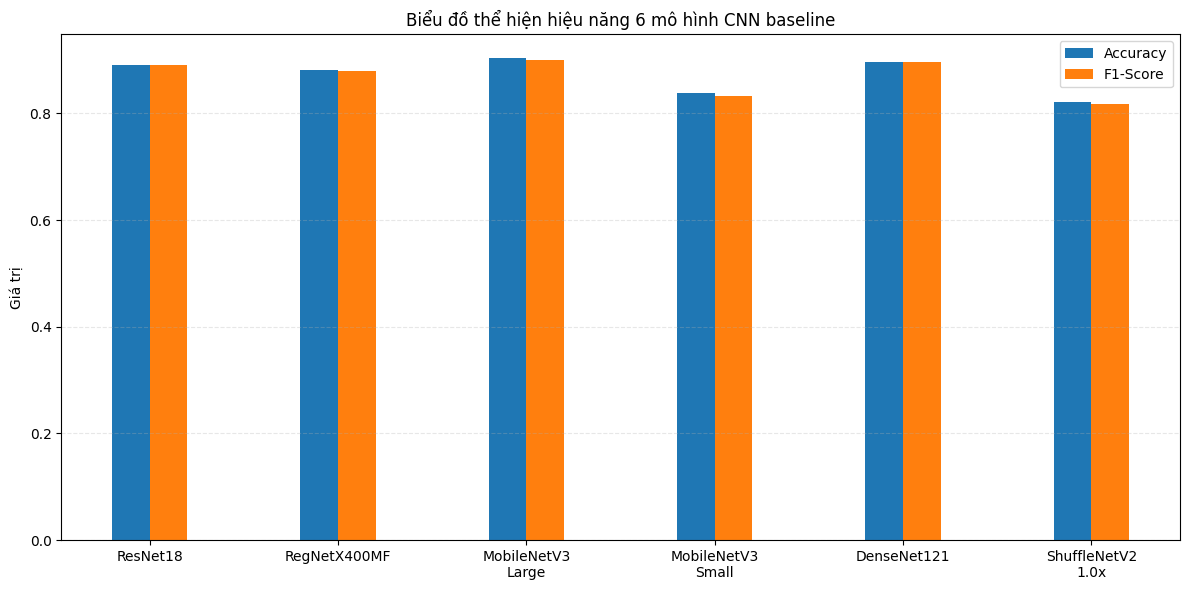
\includegraphics[width=\linewidth]{images/part-02/chap-03/sec-02/CNNBaseline.png}
    \caption{Biểu đồ thể hiện hiệu năng của 6 mô hình CNN baseline}
    \label{fig:CNNBaseline}
\end{figure}

\indent Dựa trên bảng tổng hợp và các biểu đồ thể hiện kết quả trung bình của sáu mô hình CNN baseline, có thể rút ra một số kết luận chính như sau:\vspace{-0.1cm}
\begin{itemize}[label={--}, itemsep=1pt]
    \item MobileNetV3 Large đạt được kết quả trung bình tốt nhất trong bài toán này với Accuracy đạt 0.9028 và F1-Score đạt 0.9006. Mặc dù trước đó DenseNet121 cho ra kết quả tốt nhất, điều này cho thấy sự thích ứng của mô hình MobileNet V3 Large với các tập dữ liệu khác nhau (được drop ngẫu nhiên theo random seed), làm cho kết quả của mô hình vẫn ổn định qua các lần chạy.

    \item DenseNet121, ResNet18 và RegNetX400MF đạt độ chính xác ở mức cao và khá sát nhau, lần lượt là 0.8963, 0.8907 và 0.8806. DenseNet121 vẫn thể hiện ưu thế về khả năng học đặc trưng ở từng lần chạy riêng lẻ, tuy nhiên khi xét trên kết quả trung bình, mô hình này thấp hơn MobileNetV3 Large một khoảng nhỏ. Điều này cho thấy các kiến trúc có quy mô lớn vẫn hoạt động hiệu quả, nhưng chưa hẳn là lựa chọn tối ưu nếu xét đến sự cân bằng giữa hiệu suất và chi phí tính toán.

    \item MobileNetV3 Small và ShuffleNetV2 1.0x đạt kết quả thấp hơn rất nhiều, với độ chính xác lần lượt là 0.8379 và 0.8204. Khoảng cách gần 8\% so với nhóm mô hình dẫn đầu cho thấy việc giản lược mô hình quá mức đã làm hạn chế khả năng nắm bắt các chi tiết, góc cạnh phức tạp, đặc biệt đối với các lớp dữ liệu có bối cảnh hình ảnh tương đồng.
\end{itemize}

Kết quả kiểm thử cho thấy các mô hình CNN baseline, khi chỉ sử dụng thông tin hình ảnh, có thể đạt độ chính xác xấp xỉ \textbf{0.91}. Tuy nhiên, việc khó vượt qua ngưỡng này, cùng với những hạn chế trong việc phân biệt các lớp có mức độ nhập nhằng cao (chẳng hạn như lớp \textit{le-hoi-nghinh-ong}), cho thấy sự cần thiết của việc bổ sung thêm thông tin từ hai phương thức văn bản và âm thanh.